%%%%%%%%%%%%%%%%%%%%%%%%%%%%%%%%%%%%%%%%%
% Arsclassica Article
% LaTeX Template
% Version 1.1 (10/6/14)
%
% This template has been downloaded from:
% http://www.LaTeXTemplates.com
%
% Original author:
% Lorenzo Pantieri (http://www.lorenzopantieri.net) with extensive modifications by:
% Vel (vel@latextemplates.com)
% Johan Bos (johan.bos@rug.nl)
%
% License:
% CC BY-NC-SA 3.0 (http://creativecommons.org/licenses/by-nc-sa/3.0/)
%
%%%%%%%%%%%%%%%%%%%%%%%%%%%%%%%%%%%%%%%%%

%----------------------------------------------------------------------------------------
%	PACKAGES AND OTHER DOCUMENT CONFIGURATIONS
%----------------------------------------------------------------------------------------

\documentclass[
10pt, % Main document font size
a4paper, % Paper type, use 'letterpaper' for US Letter paper
oneside, % One page layout (no page indentation)
%twoside, % Two page layout (page indentation for binding and different headers)
headinclude,footinclude, % Extra spacing for the header and footer
%BCOR5mm, % Binding correction
] {book}% {scrartcl}

%%%%%%%%%%%%%%%%%%%%%%%%%%%%%%%%%%%%%%%%%
% Arsclassica Article
% Structure Specification File
%
% This file has been downloaded from:
% http://www.LaTeXTemplates.com
%
% Original author:
% Lorenzo Pantieri (http://www.lorenzopantieri.net) with extensive modifications by:
% Vel (vel@latextemplates.com)
%
% License:
% CC BY-NC-SA 3.0 (http://creativecommons.org/licenses/by-nc-sa/3.0/)
%
%%%%%%%%%%%%%%%%%%%%%%%%%%%%%%%%%%%%%%%%%

%----------------------------------------------------------------------------------------
%	REQUIRED PACKAGES
%----------------------------------------------------------------------------------------

\usepackage[
%nochapters, % Turn off chapters since this is an article        
beramono, % Use the Bera Mono font for monospaced text (\texttt)
eulermath,% Use the Euler font for mathematics
pdfspacing, % Makes use of pdftex letter spacing capabilities via the microtype package
dottedtoc % Dotted lines leading to the page numbers in the table of contents
]{classicthesis} % The layout is based on the Classic Thesis style


\usepackage{arsclassica} % Modifies the Classic Thesis package

\usepackage[T1]{fontenc} % Use 8-bit encoding that has 256 glyphs

\usepackage[utf8]{inputenc} % Required for including letters with accents

\usepackage{graphicx} % Required for including images

\usepackage{enumitem} % Required for manipulating the whitespace between and within lists

\usepackage{lipsum} % Used for inserting dummy 'Lorem ipsum' text into the template

\usepackage{subfig} % Required for creating figures with multiple parts (subfigures)

\usepackage{amsmath,amssymb,amsthm} % For including math equations, theorems, symbols, etc

\usepackage{varioref} % More descriptive referencing
\usepackage{color}
\usepackage{listings}
\usepackage{setspace}
\usepackage{lscape}
\usepackage[authoryear]{natbib}

\usepackage{multicol}

\usepackage{algorithm} 

\usepackage{algpseudocode}

%----------------------------------------------------------------------------------------
%	DUTCH SUPPORT
%----------------------------------------------------------------------------------------

%\usepackage[dutch]{babel}    % comment out if you write your thesis in Dutch


%----------------------------------------------------------------------------------------
%	THEOREM STYLES
%---------------------------------------------------------------------------------------

\theoremstyle{definition} % Define theorem styles here based on the definition style (used for definitions and examples)
\newtheorem{definition}{Definition}

\theoremstyle{plain} % Define theorem styles here based on the plain style (used for theorems, lemmas, propositions)
\newtheorem{theorem}{Theorem}

\theoremstyle{remark} % Define theorem styles here based on the remark style (used for remarks and notes)

%----------------------------------------------------------------------------------------
%	HYPERLINKS
%---------------------------------------------------------------------------------------

\hypersetup{
%draft, % Uncomment to remove all links (useful for printing in black and white)
colorlinks=true, breaklinks=true, % bookmarks=true,
bookmarksnumbered,
urlcolor=webbrown, linkcolor=RoyalBlue, citecolor=webgreen, % Link colors
pdftitle={}, % PDF title
pdfauthor={\textcopyright}, % PDF Author
pdfsubject={}, % PDF Subject
pdfkeywords={}, % PDF Keywords
pdfcreator={pdfLaTeX}, % PDF Creator
plainpages=false,
pdfproducer={LaTeX with hyperref and ClassicThesis} % PDF producer
}


\renewcommand{\lstlistingname}{Python code}% Listing -> Python
\renewcommand{\lstlistlistingname}{List of \lstlistingname}% List of Listings -> List of Python
\definecolor{Code}{rgb}{0,0,0}
\definecolor{Decorators}{rgb}{0.5,0.5,0.5}
\definecolor{Numbers}{rgb}{0.5,0,0}
\definecolor{MatchingBrackets}{rgb}{0.25,0.5,0.5}
\definecolor{Keywords}{rgb}{0,0,1}
\definecolor{self}{rgb}{0,0,0}
\definecolor{Strings}{rgb}{0,0.63,0}
\definecolor{Comments}{rgb}{0,0.63,1}
\definecolor{Backquotes}{rgb}{0,0,0}
\definecolor{Classname}{rgb}{0,0,0}
\definecolor{FunctionName}{rgb}{0,0,0}
\definecolor{Operators}{rgb}{0,0,0}
\definecolor{Background}{rgb}{0.98,0.98,0.98}




 
\lstdefinestyle{mystyle}{
numbers=left,
numberstyle=\footnotesize,
numbersep=1em,
xleftmargin=1em,
framextopmargin=10em,
framexbottommargin=2em,
showspaces=false,
showtabs=false,
showstringspaces=false,
frame=l,
tabsize=4,
% Basic
basicstyle=\ttfamily\small\setstretch{1},
backgroundcolor=\color{Background},
language=Python,
% Comments
commentstyle=\color{Comments}\slshape,
% Strings
stringstyle=\color{Strings},
morecomment=[s][\color{Strings}]{"""}{"""},
morecomment=[s][\color{Strings}]{'''}{'''},
% keywords
morekeywords={import,from,class,def,for,while,if,is,in,elif,else,not,and,or,print,break,continue,return,True,False,None,access,as,,del,except,exec,finally,global,import,lambda,pass,print,raise,try,assert},
keywordstyle={\color{Keywords}\bfseries},
% additional keywords
morekeywords={[2]@invariant},
keywordstyle={[2]\color{Decorators}\slshape},
emph={self},
emphstyle={\color{self}\slshape},
captionpos=b, 
}
 
\lstset{style=mystyle}

\def\vl{\\[9pt]}
 % Include the structure.tex file which specified the document structure and layout


%----------------------------------------------------------------------------------------
%	HYPHENATION
%----------------------------------------------------------------------------------------

\hyphenation{Fortran hy-phen-ation} % Specify custom hyphenation points in words with dashes where you would like hyphenation to occur, or alternatively, don't put any dashes in a word to stop hyphenation altogether



%----------------------------------------------------------------------------------------
%	TITLE AND AUTHOR(S)
%----------------------------------------------------------------------------------------

\title{\normalfont\spacedallcaps{title}} % The article title

\author{\spacedlowsmallcaps{author}} % The article author(s) - author affiliations need to be specified in the AUTHOR AFFILIATIONS block

\date{} % An optional date to appear under the author(s)

%----------------------------------------------------------------------------------------

\begin{document}

%----------------------------------------------------------------------------------------
%	HEADERS
%----------------------------------------------------------------------------------------

%\renewcommand{\chaptermark}[1]{\markright{\spacedlowsmallcaps{#1}}} % The header for all pages (oneside) or for even pages (twoside)
%\renewcommand{\subsectionmark}[1]{\markright{\thesubsection~#1}} % Uncomment when using the twoside option - this modifies the header on odd pages
%\lehead{\mbox{\llap{\small\thepage\kern1em\color{halfgray} \vline}\color{halfgray}\hspace{0.5em}\rightmark\hfil}} % The header style

\pagestyle{scrheadings} % Enable the headers specified in this block


%----------------------------------------------------------------------------------------
%	TITLE PAGE
%----------------------------------------------------------------------------------------

\hypersetup{pageanchor=false}
\begin{titlepage}
\thispagestyle{empty}
\begin{figure}[h!] %  figure placement: here, top, bottom, or page
  
\includegraphics[width=4in]{ruglogo}
\end{figure}

\begin{center}
\vspace{30 mm}
\begingroup \linespread{1,75} \selectfont
\textsc{\LARGE Context \& Common Knowledge}\\
\textsc{\Large Using an entity linker and knowledge base to detect hard entities in need of an explanation}\\[1,5cm]
\endgroup

Wessel Poelman\\[2,5cm]

\end{center}
\vfill
\textbf{Bachelor thesis}\\
Information Science\\
Wessel Poelman\\
S2976129\\
\today
\end{titlepage}
\hypersetup{pageanchor=true}



%----------------------------------------------------------------------------------------
%	ABSTRACT
%----------------------------------------------------------------------------------------

\pagenumbering{roman}
\chapter*{Abstract}
\markboth{Abstract}{Abstract}
\addcontentsline{toc}{chapter}{Abstract}

% This is what Kenneth K. Landes says about abstracts: ``The abstract is
% of utmost importance for it is read by 10 to 500 times more people
% than hear or read the entire article. It should not be a mere recital
% of the subjects covered, replete with such expressions as \textit{is
%   discussed} and \textit{is described}. It should be a condensation
% and concentration of the essential qualities of the paper.''. In other
% words, it should comprise the goal of the thesis, describe the problems, the
% method used to solve them, the obtained results, and what consequences
% the results have (conclusions). Try to fit the abstract on one page (remember: it is abstract, not an essay).

Current automatic text simplification research is not very focused on named entities.
These can definitely be a source of difficulty for a reader.
A grammatically simplified sentence with a hard entity can still be difficult to understand.
This project focusses on explaining difficult named entities in texts \textit{when it is needed}.
The following question is answered: \textit{How can a system decide if named entities in a text need an explanation?}
This is done by using an entity linker and knowledge base to retrieve information about an entity.
The decision, if an explanation is needed or not, is made by using a list of `common knowledge' entities and the context of a given entity in a text.
Human annotators got the same task of making this decision and agreed in 76\% of cases with the system.
In conclusion, by comparing the context of a named entity to information in a knowledge base and by counting entity occurrences in a suitable corpus to determine which are common knowledge, a system can make a decent decision if a named entity needs an explanation or not.\\

The source code is available at: \url{https://github.com/WPoelman/thesis_is}

% 1. Waarom en waarover je de scriptie hebt geschreven
% 2. Hoe je het onderzoek hebt uitgevoerd
% 3. Wat uit je onderzoek is gebleken
% 4. Wat je resultaten betekenen
%
% Presenteer je conclusie (oftewel het antwoord op je hoofdvraag).
% Houd het kort door alleen in te gaan op het antwoord op je hoofdvraag en specifiek aan te kondigen wat je conclusie is (bijv. “de conclusie is daarom…”).



%----------------------------------------------------------------------------------------
%	TABLE OF CONTENTS & LISTS OF FIGURES AND TABLES
%----------------------------------------------------------------------------------------
\clearpage
\setcounter{tocdepth}{3} % Set the depth of the table of contents to show sections and subsections only
\tableofcontents % Print the table of contents

%\listoffigures % Print the list of figures (optional, only if you have many figures)

%\listoftables % Print the list of tables (optional, only if you have many tables)

%\lstlistoflistings



%----------------------------------------------------------------------------------------
%	Preface
%----------------------------------------------------------------------------------------

\chapter*{Preface}
\markboth{Preface}{Preface}
\addcontentsline{toc}{chapter}{Preface}
% The preface usually contains information that has nothing to do with
% the contents of the thesis. It has a personal character, and is
% written in the first person. It could contain personal circumstances,
% the context in which the thesis has been written, a description of the
% assignment, information about the author, and relations to other
% reports or theses. It is also the place to thank people that helped
% you, including your well-deserved supervisor!

This thesis was quite special for me.
Almost exactly a year ago I completed the bachelor Communication and Information Sciences.
While that was definitely interesting, I knew it was not what I wanted to pursue a career in.
The Information Science field suits me a lot better and now I know I want to go further in the Information Science / Computer Science field.

The current project involved of a lot of trial \& error and experimentation, which caused some headaches.
When I found a configuration of parts that worked and combined them all, it was very satisfying and the fun part started.
I enjoyed the building of the system the most and looking at the interesting, strange and sometimes funny output from it.

I am quite happy with the results considering it is something that (to my knowledge and research) has not been done before.
Before starting this thesis I hardly knew that the field of `automatic text simplification' existed.
While working on this thesis I realized it is a surprisingly broad and interesting research area.

I would like to thank my supervisor Gertjan van Noord.
Compared to my CIS thesis supervisor, there was not a lot of interaction, but the talks we had were useful and helped with some tough parts.
This topic was also well suited for trying things on your own and did not need hand holding.
I would also like to thank my mother for her proof reading (second time!) and general support.\\

I hope you enjoy reading this thesis.\\

Wessel Poelman

%----------------------------------------------------------------------------------------
%	INTRODUCTION
%----------------------------------------------------------------------------------------

\chapter{Introduction}
\pagenumbering{arabic}
% The introduction is the first chapter of your thesis. Every reader
% needs an introduction to the topic of your thesis (it doesn't need to
% be called ``Introduction''). It is not always easy to write a coherent
% and comprehensible introduction: it requires practice. It sometimes
% makes sense to write the other chapters first, but this also has the
% risk that many things are taken for granted for the reader.  The
% introduction provides that stage for the topic of the thesis, and
% usually has three key parts \citep{Nederhoed:2010}:

% \begin{enumerate}
% \item Which research questions the thesis is providing answers to (or trying to);
% \item Why answers are given to these questions (motivation);
% \item How the answers are given (structure).
% \end{enumerate}

% It is not necessary to write a very long introduction. Try to make it
% snappy with a catchy opening that arouses interest of the reader --
% often the first sentence decides whether a reader is to read your
% report or not. There are many ways of doing this \citep{Nederhoed:2010}.

% The rest of the thesis usually has a fixed structure. First of all
% more about the theoretical background is given in a separate chapter
% (unless this is very brief -- in which case it could be part of the
% introduction). Then a description of the data material is provided:
% this could be done in a separate chapter or part of the method
% chapter. The method chapter gives a detailed overview of the used
% approach is given, and usually this chapter is called \textit{Method},
% \textit{Methodology}, \textit{Method and Tools}, or something similar.

Determining the difficulty of a text or sentence is not an easy task.
Intuitively we have some ideas about what makes a text simple or hard.
To explain or pinpoint what causes this, is not as trivial as it might seem.
Is text difficulty caused by word choice, sentence length, topic, structure?
Is it a combination of all of the above? As \citeauthor{shardlow2014} put it in a 2014
automatic text simplification overview article:

\begin{quote}
  Simplicity is intuitively obvious, yet hard to define. (p.59)
\end{quote}

This intuition is straightforward for humans, but not for a computerprogram.
Making the decision if a text is difficult or not and what to do about it, can be done on many different levels.
Altering the size of a text, rewriting sentences, restructuring information, replacing difficult terms with simpeler variants to name a few \citep{alva2020}.
One of these levels is explaining difficult parts of a text.
With this approach, the text is not made shorter to decrease the amount of information, but longer to provide more clarity and increase understandability.
Or, more concisely put by \citeauthor{alva2020} in their automatic text simplification overview article from 2020:

\begin{quote}
  (\ldots) simplifying a text could also involve further explaining complex terms or concepts.
  This is not merely replacing a word or phrase for a simpler synonym or its definition, but to
  elaborate on the concept in a natural way that keeps the text grammatical,
  is meaning preserving, and is simple. (p.177)
\end{quote}

This quote highlights two important challenges of explaining `complex terms or concepts'.
First, a resource is needed from which to create or get explanations.
Second, a decision has to be made which terms are in need of an explanation.
To solve the first problem there are numerous large and open resources (knowledge bases) that can be used for this.
Wikipedia is a great example of a general knowledge base.
For more domain specific knowledge there are also various resources available.
The second problem is harder to solve.
To illustrate, this problem has an effect on all aspects of the previous quote.
Every recognized term from a knowledge base could be explained, this would `elaborate on the concept', but not in a `natural way'.
There needs to be a method of deciding when an explanation is \textit{needed}.
This also touches on the other points from the quote.
It is hard to imagine a grammatical or readable text in which every term is explained.
This would lead to the opposite of the goal of making the text simpler.
The question is \textit{how} a system can make a decision when an explanation is needed or not.

The scope of this question is too broad.
In practical terms, what is considered a `term or concept'?
This could be individual words, sentences or even chapters.
The level of detail needs to be such that the term is easy to find in a knowledge base and has a short and simple explanation.
This touches on several natural language processing fields, the most useful being `entity linking', which comes close to the goal here.
This field focusses on automatically recognizing entities from a knowledge base in a given text.
This is a good starting point, but knowledge bases, such as Wikipedia, contain entities that are not suitable for simplifying using explanations.
Take articles for individual years or dates for example.
These most likely do not need explaining and how can a year even be `explained'?
To restrict the question, this project focusses on \textit{named entities}.
These include persons, geographical locations, brands or organizations.
Luckily, entity linkers and general knowledge bases predominantly target named entities.
In automatic text simplification research, named entities are also somewhat neglected.
A good opportunity to try something new.
The main research question is the following:

\begin{quote}
  How can a system decide if named entities in a text need an explanation?
\end{quote}

To make that decision, two factors have to be taken into account: context \& common knowledge.
A named entity can be explained by the context of the sentence or text it occurs in.
Some entities are not explained in texts because they are considered to be common knowledge.
A named entity such as `Amsterdam' is generally not explained in texts.
Two sub questions address these factors:

\begin{quote}
  \begin{enumerate}
    \item How can context be captured and used to decide if a named entity needs an explanation?
    \item How can common knowledge be captured and used to decide if a named entity needs an explanation?
  \end{enumerate}
\end{quote}

To answer these questions, a system was made that generates explanations for named entities, makes a choice if the explanation is needed and annotates an input text with the needed explanations.
The system also produced versions with and without explanations of all sentences in which entities were recognized.
These were shown to human annotators who had to make the same `needed' or `not needed' decision.

\chapter{Background}
% In this chapter (you are free to give it a different name) you include
% previous research that has been done in this field: an overview of the
% state-of-the-art, with appropriate references, such as
% \citep{task11-2015}. Also explain how your work differs from what has
% been done before, or how it extends previous work.

% The \texttt{natbib} packages offers many way to cite related work, for
% instance with parentheses \citep{Nederhoed:2010}, or without, as
% explained in \citet{Nederhoed:2010}. Multiple citations are also
% possible \citep{Nederhoed:2010,task11-2015}.
This chapter outlines where the current project ties into existing `automatic text simplification using explanations' research.
Next, the role of named entities \& entity linkers is described.
Finally, some disambiguation methods used by entity linkers are explained to illustrate the approach of dealing with the context of an entity in a text.

\section{Simplifying using explanations}
As stated in the Introduction, explaining difficult terms is one of many ways to simplify a text.
Some research has been done, but ``this is an important research area in SS (sentence simplification) where limited work has been published'' \citep{alva2020}.
Two fields in this area will be highlighted: \textit{healthcare} and \textit{reading assistance}.

\subsection{Healthcare}
Healthcare is a field where hard terms contributing to the difficulty of a text is clearly visible.
A decent amount of research has gone into explaining difficult medical terms.
The systems developed for this often have a secondary screen or interface showing the explanation \citep{alfano2020,alsheref2020,qenam2017}.
A user needs to explicitly point out to the system which term they want explained.
These systems use vocabularies of medical terms with so called `consumer explanations' to find an explanation for a given term.
These explanations are manually created by experts.
This research and the systems are highly domain specific and have some drawbacks.
The first being the fixed nature of the vocabularies.
When a new term is added, the vocabulary needs to be updated.
An expert needs to manually create a new explanation for that term.
The same problem applies when updating existing terms with new explanations.
This means that the system is quite hands on when it comes to extendibility and limited in the terms it can find.

The current project, while not applied to healthcare specifically, uses Wikipedia as a general knowledge base.
The advantage of this, is that the system retrieves information in real time.
At the moment of generating the explanation, the information about an entity is as recent as the last update on that entity's article.
Another advantage is that, theoretically, all entities in the Wikipedia database can be explained.
This is, however, limited by the recognition of those terms and the language used.
This project is mainly limited by the entity linker.
This real time approach is more extendible than the fixed vocabulary.
The downside of using Wikipedia is that the quality of the information is not guaranteed.
Expert explanations in the vocabulary approach are likely more consistent than the open editing nature of Wikipedia.

Aside from the vocabularies, the systems in healthcare use an all or nothing approach.
Both the systems that use an external screen for the explanations and the systems that insert them into the source text overlook an essential part of explaining a term, which is context.
The external method somewhat solves this by letting the user choose what they want explained.
If the user understands the term, they simply do not click on it.
This is a convenience of the design, rather than a solution to the problem.
If a term gets an inline explanation, but gets naturally explained in the next sentence, it arguably makes the text more confusing.
The point of the current project is to explain a term only when it is \textit{needed}.
If a term gets explained in context, the system should be smart enough to \textit{not} explain it and vice versa.
What is considered `context' will be clarified later.

As mentioned, a lot of the findings in the healthcare text simplification field are quite domain specific.
Some of the discoveries are more broadly applicable though, such as a study from \citeauthor{gu2018} from 2018.
This study looked at the use of parentheses when providing explanations in texts.
The main experiment consisted of inserting the explanation in the text and surrounding the difficult term with parentheses, or vice versa.
They showed that for already simple texts, it is best to enclose the explanation with parentheses and in difficult texts, the other way around.
The current project uses online news articles, which are not considered to be difficult texts (more on this later).
This is why the system in the current project encloses the explanations in parentheses behind the term that needs to be explained, following the recommendations of \citeauthor{gu2018}.

\subsection{Reading assistance}
There have been some attempts at generating explanations for reading assistance.
A study done by \citeauthor{watanabe2010} from 2010 looked at providing explanations for terms in web texts through the use of a browser plugin.
The user could click on terms and a highlighted popup with an explanation would appear.
Something similar has been done by \citeauthor{eom2012} in 2012 to disambiguate words for struggling readers and by \citeauthor{azab2013} in 2013 to help people with learning a foreign language.
All three studies have some major drawbacks.
They use tools or interfaces that need to be open outside of the actual text during reading.
This arguably hinders the reader as they need to switch to the system and back to the text while reading.
That `break' in the reading process could result in needing to reread a section or needing to find where they were.
While these seem like minor inconveniences, the tools are aimed at struggling readers.
Any additional obstacles only make reading harder.
Additionally, the systems are reliant on user input, usually in the form of clicking on text elements.
This also interrupts the reading process.
Finally, as with the healthcare systems, there is no regard for context, it is all or nothing.
The current project aims to provide explanations for named entities \textit{when needed}, based on context and common knowledge.
Explanations are inserted into the original text and sourced from a general knowledge base.
No external system needs to be open alongside reading the text.

\section{Named entities}
In current automatic text simplification research, named entities are somewhat neglected.
In the previously mentioned paper by \citeauthor{alva2020} from 2020, for example, a sentence splitting model is presented that ``strips off named entities and properties'' (p.164).
When replacing difficult words with simpeler synonyms, named entities are often discarded or replaced by a dummy word in order to reduce the size of vocabularies \citep{nisioi2017,alva2020}.

Considerable research is dedicated to shortening sentences or grammatically restructuring texts.
These approaches are important when simplifying, but a simplified sentence with difficult terms is not necessarily simple.
Named entities are a good candidate to simplify because they can generally be explained in a couple of words.
Take for example a recent news article from the University of Groningen about Ezinge\footnote{\url{https://www.rug.nl/news/2020/10/ezinge-revisited}}.
In the article there is no clear explanation of what Ezinge is.
This is assumed to be common knowledge and for most people from northern provinces of the Netherlands, this would probably be true.
This is, however, not guaranteed and a simple inline explanation in the first sentence could help with understandability:

\begin{quote}
  \textit{Dutch:} De opgraving in de wierde van Ezinge \textbf{(Gronings dorp)}, tussen 1923 en 1934 uitgevoerd door prof. Albert Egges van Giffen, behoort tot de bekendste opgravingen in de geschiedenis van de Nederlandse archeologie.\newline
  \textit{English:} The excavation in the Mound of Ezinge \textbf{(village in Groningen)}, carried out between 1923 and 1934 by Prof. Albert Egges van Giffen, is one of the most famous excavations in the history of Dutch archeology.
\end{quote}

Named entities themselves are a large research area within natural language processing.
Entity linking, for example, looks at recognizing \& disambiguating named entities in a text and linking them to a knowledge base \citep{shen2015,vanhulst2020}.
All these areas are important for the current project.
One of the main components of the system is an entity linker.
Entity linkers are mostly used to assist components of information retrieval systems \citep{delpeuch2019,vanhulst2020}.
General entity linkers have not been used in text simplification applications using explanations.
The discussed healthcare systems do link a term to an explanation, but they do not use a \textit{general} knowledge base.
Disambiguation is also rarely needed in those systems.
Some of the reading assistance systems do use a form of entity linking, but there the system does not need to find the entities in the text, the user does that by clicking.

Current state of the art entity linkers use a variety of knowledge bases and approaches.
For the current project a Dutch, pre-trained entity linker is needed.
There are some recent attempts at Dutch entity linkers\footnote{This project started with experiments using:\newline
  - DAC from the Dutch National Library \url{https://github.com/KBNLresearch/dac} \newline
  - An entity linker for historical Dutch articles from the VU Amsterdam \url{https://github.com/cltl/entity-identification-from-scratch}}, but they are not as well maintained or recent as their English counterparts.
Pre-trained systems for Dutch are even harder to come by.
Additionally, some are too domain specific, targeting only historical documents for example.
For this reason, the system used in this project is DBPedia's Spotlight with their 2016 Dutch language model, created by \citeauthor{daiber2013} in 2013 (updated in 2016).
This is not a state of the art system, but it provides a clear and usable API and comes with a pre-trained model.
Spotlight provides entity recognition, disambiguation and linking using DBPedia as a knowledge base.
The main knowledge base this project uses is Wikipedia.
DBPedia provides methods to convert to Wikipedia entries.
More detailed information on Spotlight will be provided in the Method chapter.

\section{Inspiration from disambiguation methods}
The disambiguation methods in entity linkers give a good starting point of how to look at the context of a named entity.
Disambiguation involves looking at which variant of an entity is the right one \textit{given the context}.
For example, the sentences \textit{`the Miami Heat beat the LA Clippers last weekend'} and \textit{`the Miami heat was tough for farmers this year'} both contain the possible named entity `Miami heat', thus being ambiguous.
When looking at the context, the first sentence has another basketball team in it.
When a system has access to a knowledge base, it can use that information to guess that the first one is probably referring to the basketball team and the second to weather conditions.

This process is often done by providing a confidence score of which variant the system thinks is the closest.
There are many disambiguation methods and techniques.
The current project has been influenced by methods that leverage a knowledge base to figure out what is happening in the context of an entity.
Specifically, the current system looks at how \textit{different} the context is to information in the knowledge base.

Looking at that context can be done in several ways, such as word vectors (embeddings), counting previous mentions or using the `relatedness' of Wikipedia links \citep{delpeuch2019,ma2019,vanhulst2020}.
Disambiguation algorithms and methods often do not use long form `semantic' information from a knowledge base.
They use data that allows for graph calculations or to enhance features of an entity \citep{rao2013}.
This data is often used as machine learning features.
These include: categories, identifiers, edges of related entities in graph representations or popularity.
There is, however, a lot more information in knowledge bases that could be used in analyzing context.
Take Wikipedia for example, short descriptions, summaries, even full articles provide a lot of information.
The system in the current project uses this type of information to make the decision if an explanation is needed.

In a paper by \citeauthor{vanhulst2020} from 2020, they used special \verb+Wikipedia2Vec+ word and entity embeddings.
These encoded word embeddings as well as Wikipedia metadata.
A context window of 50 words surrounding an ambiguous entity was used.
This context was transformed to embeddings using \verb+Wikipedia2Vec+ and similarity was calculated between the context and entity embeddings.
Other steps were used, but this particular method can also be used in deciding if an entity needs an explanation.
In some way, disambiguation already gives information about how well the entity `fits' in its context by using embeddings.
This is not the same as explaining the entity in the context, but it does provide a starting point.
The current project uses a context window consisting of the sentence in which the entity occurs and the sentences left and right from it.
The context window is described further in the Method Chapter.

The current system uses the first sentence of a Wikipedia abstract from the knowledge base for comparison.
This is done in order to keep the size of the context window relatively the same as the size of the information from the knowledge base.
This also generally provides the most information about an entity in a short and succinct way.
The abstract, along with the description of the entity, get transformed into word embeddings and compared to the context, similar as what \citeauthor{vanhulst2020} did.
When this information from the knowledge base is \textit{different enough} from the context, an explanation is needed. The specific approach and how the system deals with common knowledge is discussed in the Method Chapter.

The following chapters explain the data used in the project, the validation procedure, the specifics of the system and finally the results and conclusions.

\chapter{Data and Material}
\section{Collection}
\subsection{Dataset}
The corpus used for this project is the \verb+DutchWebCorpus+, created by Wietse de Vries.
This dataset consists of all online news articles from 2015 to mid 2019 from four major
Dutch news outlets: NOS, NU.nl, de Telegraaf \& de Volkskrant. The total number of
articles is roughly 990.000, totalling more than 270 million words.
This dataset is chosen because news articles contain a large number of named entities.
Online news articles are also of suitable length.
The system uses a decently sized context window to make the decision.
Named entities in short texts, such as tweets, generally do not have sufficient context.
News articles are also suitable because of their textual structure.
Since they are not that long, they have to be compact and concise with presenting information.
If the author thinks a named entity needs an explanation, it has to be done quite close to the first time that named entity is mentioned.
Simply because there is not enough space to do this in a later chapter for example.
Furthermore, the structure generally does not use distant explaining of terms.
With books or long form articles, footnotes or registers can be used to explain complex terms `far away' from the sentence they occur in.
Online news articles do not have this luxury. The dataset is used for two purposes:
\begin{itemize}
  \item Extracting information about all named entities to capture which named entities are common knowledge.
  \item To annotate texts with explanations and present the intermediate results to validate the choices of the system.
\end{itemize}

\subsection{Entity linker}
As mentioned in the Background Chapter, the entity linker used is DBPedia's Spotlight.
This is by no means a state of the art entity linker, but this is not a big issue for the current project.
The main focus is the decision if a named entity needs an explanation, not if every entity is recognized.
The Method chapter elaborates on the configuration and use of Spotlight.

\subsection{Knowledge base}
The knowledge base used is Wikipedia.
For the purposes of this project, it is a good and large resource for general information about named entities.
It also has an open API which serves two functions:

\begin{itemize}
  \item Retrieving an explanation for a given entity.
  \item Retrieving information about the entity to compare its context to.
\end{itemize}
\newpage

\section{Annotation}
% Specify too in as much detail as possible your labels, data features
% you decide to use as indicators of your labels, and any annotations
% you need additionally.
In the project there are two steps where texts are annotated, by the system and by human annotators.

\subsection{System}
The system receives an input text and decides which named entities need an explanation.
When needed, the system inserts the explanation between parentheses behind the entity in question.
The final output text is the original text with explanations.
During this process, it produces detailed intermediate, annotated data.
It creates a version of the sentence with and without the explanation for all named entities it recognized.
These include the context sentences the system also used for the decision.

\subsection{Human annotators}
The human annotators got to see two versions of the entity in context, with and without explanation.
Figure \ref{figure:validation} shows an example of this.
The annotators got instructions to choose the version which makes the text more understandable and `simple'.
In other words, they needed to choose the one where the explanation was needed and supported the understanding of the text.
The labels used were `with explanation' and `without explanation'.
The full instructions can be found in the \verb+validation.html+ file in the GitHub repository.

\begin{figure}[hbtp]\centering
  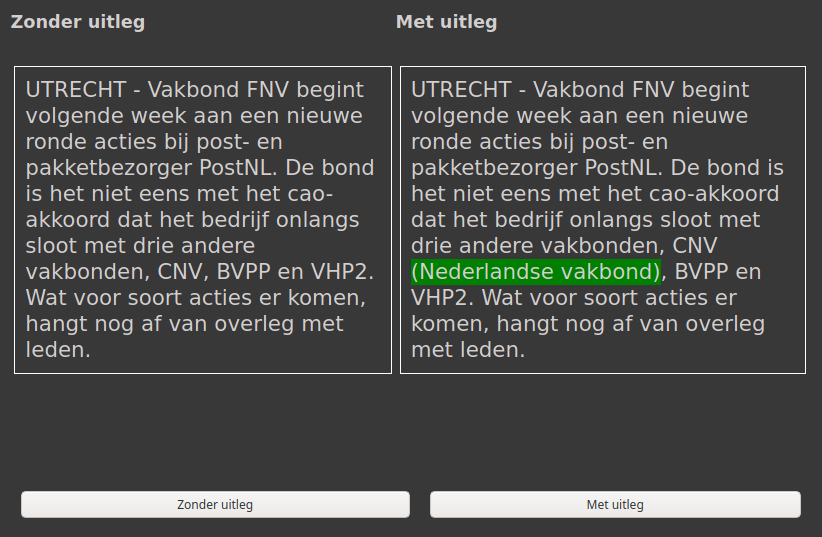
\includegraphics[width=4in]{validation_example.png}
  \caption{Example of what the human annotators needed to choose between.\label{figure:validation}}
\end{figure}

\section{Processing}
% Describe the way you intend to process your data as explicitly as possible.
The final data gets processed and analyzed in several steps.
First, the output of the system is analyzed to find interesting examples and inaccuracies.
This is done by looking through the output texts, the scores assigned to the decisions and the intermediate output of the system.
Second, the human annotated data is compared with the system annotated data.
This consists of calculating the inter-annotator agreement for the human annotators and the agreement of the system and human annotations.

\chapter{Method}
% Explain and motivate here the general approach you adopt in order to
% execute and evaluate your research (i.e. to answer your research
% question) successfully.  In your final thesis all the details of your
% method (machine learning, rules, algorithms, features, and so on will
% end up here). A good description allows other researcher to reproduce
% your results! Sometimes a picture helps to explain things
% (Figure~\ref{figure:example}) -- see \citet{Nederhoed:2010} how to
% include figures in your text and how to refer to them.

% \begin{figure}[hbtp]\centering
%   
\includegraphics[width=4in]{ruglogo}
%   \caption{This is an example of a figure with a proper caption.\label{figure:example}}
% \end{figure}
This section first explains the approaches used for the sub questions.
Next, the individual components of the system are clarified, along with a full walk through of the system.
Finally, the validation process is outlined.

\section{Context}
The first sub question:
\begin{quote}
  How can context be captured and used to determine if a named entity needs an explanation?
\end{quote}

A named entity can be explained in the sentence it occurs in or in the surrounding text.
As mentioned, in news articles this explaining is often close to the first mention of the entity.
News articles do not have the length to explain an entity later on.
Because of this, the context window used is the sentence the entity occurs in (S = sentence), one sentence before that (L = left sentence) and one after (R = right sentence).
L and R do not always exist if S is the first or last sentence of an article.

The system needs compare the context (LSR) to something to decide if an explanation is needed.
This is where the knowledge base comes into play.
The following information about the entity is collected from the Wikipedia API:
\begin{multicols}{2}
  \begin{itemize}
    \item The \verb+description+ field (D)
    \item The \verb+abstract+ field (A)
  \end{itemize}
\end{multicols}

D is a short description of the entity.
For example, Amsterdam has `capital of the Netherlands' as its description.
The project uses the Dutch version of Wikipedia, but the approach is not language dependent.
D is used in evaluating the context and also serves as the explanation that is inserted into the text.

The abstract is (a shortend version of) the first paragraph of the Wikipedia article about the entity.
Here, the system only selects the first sentence (A).
This is done because the first sentence of a Wikipedia article generally presents the most important information about the topic in a compact and direct way.
For the purposes of this project, A can be considered the longer and more detailed version of D.

D and A are both used because, while D can give a decent amount of information about the entity, it is limited in scope.
A gives a lot more information and casts a wider net of how the entity could be explained in the context.
The larger amount of information in A does along the risk of noise, more on that later.
Next, some pre-processing is done for L, S, R, D and A:

\begin{itemize}
  \item Stop words are removed
  \item Mentions of the named entity are removed
\end{itemize}

When `context' is mentioned in this section, it refers to a combination of the cleaned versions of L, S \& R.
From now on D and A also refer to their cleaned versions.
This cleaning is done in order to prevent `tainting' the similarity between L, S \& R and D \& A.
Stop words can wrongly make it seem like two very different sentences are quite similar.
The entity is removed because it says nothing about \textit{it being explained}, it is not part of the `context'.

Next, L, S, R, D \& A are converted to word embeddings using the large Dutch language model (\verb+nl_core_news_lg+) from Spacy\footnote{\url{https://spacy.io/models/nl\#nl_core_news_lg}}.
Spacy uses FastText \citep{bojanowski2016} for their word embeddings.
These are trained on web texts and Wikipedia, which is conveniently appropriate.
In Spacy terms, L, S, R, D \& A are \verb+Spans+ of \verb+Tokens+, which roughly means a \verb+collection+ of \verb+words+.
These \verb+Tokens+ contain the word embedding vector for themselves and \verb+Spans+ can access these.

Finally, the similarity between the context and D \& A is computed and a score is assigned.
The built in Spacy method \verb+similarity+ on \verb+Spans+ is used.
This method calculates the cosine similarity of the average of the word vectors in the two \verb+Spans+ that are being compared.
The advantage of using this method is that it captures a lot of semantic information.
This means that word order, synonyms or structure do not matter that much.
It is all captured quite well by the individual word embeddings and the average of those embeddings.
For example, if the entity is `Washington D.C.', S is 'city America' and D is 'capital USA', the similarity between S and D is 0.63.

Calculating the similarities is done in pairs, consisting of an item from the context and D or A.
These get summed for D and A and averaged to the number of items in the context.
As mentioned, L and R might not exist and this deals with the possible difference in context length.
Finally, a weight is assigned to the average similarity of D and A.
This is done because (the uncleaned version of) D is inserted into the text.
If that similarity is high, it is likely that the entity is explained in the context.
A contains more information and is thus more prone to noise having an effect on the similarity, even when stop words are removed.
With some experimentation the final weights are 0.7 for D and 0.3 for A.
The sum of these is the final score and a threshold of 0.5 has been used.
This means that the context is \textit{not similar enough} to D and A with a score of 0.4.
The entity, therefore, requires an explanation.
With a score of 0.6, the context is \textit{similar enough} to D and A.
The entity is likely already explained in the context and does not need an explanation.
The pseudocode in Algorithm \ref{figure:context} shows the process of calculating the score with all three items present in the context.

\begin{algorithm}
  \caption{Pseudocode for producing similarity score\label{figure:context}}
  \begin{algorithmic}[1]
    \State $contextItems = [L, S, R]$
    \State $knowledgeItems = [D, A]$ \\

    \For {$contextItem = [L, S, R]$}
    \For {$knowledgeItem = [D, A]$}
    \State $x$ = average of word vectors $contextItem$
    \State $y$ = average of word vectors $knowledgeItem$ \\

    \State Compute cosine similarity of $x$ \& $y$
    \EndFor
    \EndFor \\

    \State $avgD$ = Sum similarities grouped by $D$ / length of $contextItems$
    \State $avgA$ = Sum similarities grouped by $A$ / length of $contextItems$\\

    \State $finalScore = (0.7 * avgD) + (0.3 * avgA)$
  \end{algorithmic}
\end{algorithm}

\section{Common knowledge}
The previous method tries to capture knowledge about the entity \textit{inside} the text to decide if the explanation is needed.
That decision is fine if the entity gets explained enough in the context window.
When an entity does not get explained enough, however, the system would always decide to insert the explanation.
This does not take the reason for not explaining an entity into account, which often is \textit{common knowledge}.
The previously mentioned example of Amsterdam illustrates this.
Especially in news articles, this entity can be considered common knowledge.
Something similar can be said about large sports clubs, celebrities, countries, world leaders, artists, brands and so on.
The approach to tackle the second sub question is explained here.
\begin{quote}
  How can common knowledge be captured and used to decide if a named entity needs an explanation?
\end{quote}

Since the dataset contains almost a million recent news articles, spanning almost four years, from four different sources, it is a suitable place to look for common knowledge.
To 100\% decide if a named entity is considered `common knowledge', is almost impossible since it dependens on a lot of different factors.

The method used in this project is the straightforward approach of counting all occurrences of named entities.
This is done using the Spacy NER (named entity recognition) model, also from \verb+nl_core_news_lg+.
This model does not have state of the art performance, but is good enough for the purposes of this project.
The process of counting was done by running the entire corpus of roughly one million articles through this NER model and keeping a count of all entities it encountered.
The entities were normalized to all lowercase to make the count more accurate.
This resulted in a dictionary of 1.826.103 unique entities.
The model was not restricted in categories it was allowed to find.
This included entities such as dates and percentages.
This was done on purpose since the approach of the other components was not finalized at this point.
Categories other than named entities might have been useful as well.
The resulting dataset has been added to the GitHub repository of this project\footnote{The files: \textit{all\_entity\_counts.csv} \& \textit{all\_entity\_counts.pickle}}.
It took a long time to create and might be useful for other projects.
As an illustration, Table \ref{table:entity_counts} shows the ten most common entities and their counts.

\begin{table}[hbtp]\centering
  \caption{Top ten most frequent entities in the DutchWebCorpus\label{table:entity_counts}}
  \begin{tabular}{cc}
    Lowered entity & Occurrences \\
    \hline
    twee           & 353.610     \\
    eerste         & 329.076     \\
    nederland      & 278.561     \\
    nederlandse    & 200.816     \\
    amerikaanse    & 187.679     \\
    drie           & 171.847     \\
    tweede         & 148.224     \\
    amsterdam      & 135.706     \\
    één            & 130.717     \\
    vrijdag        & 106.078     \\
  \end{tabular}
\end{table}

Next, a cutoff point had to be chosen for when an entity was considered `common knowledge'.
After experimenting, the cutoff was set at the top 1\% most common entities.
This created a list of 18.261 entities, with the least frequent entity occurring 118 times.
If the system encounters an entity from that top 1\%, it knows it does \textit{not} need to explain it.
Entities are first lowered before checking if they are present in the list\footnote{A Python set is used in practice for efficiency, but a `list' is easier to imagine here.}.
In the \verb+support+ folder of the source code, the scripts for creating this list are included.
Another cutoff point can easily be chosen.

When looking through the list, the following categories of named entities are very common: cities, countries, athletes, world leaders, technology and clothing brands, artists and large companies.
This captures quite a lot of common knowledge.
The only `type' of named entity that is not captured well with this method, is historic figures / events.
These generally do not occur in news articles, unless a museum or something similar is mentioned.
In this project the same dataset is also used for annoting, common knowledge from the \verb+DutchWebCorpus+ is therefore captured well enough.
This method is specific to a corpus and use case and might not be generalizable to other texts.

\section{System components}
This section will provide a walk through the system, starting with an article from the corpus as input.

The article text first gets sent to the entity linker Spotlight, which is configured to look for names, organizations, persons and places\footnote{Specifically the following DBPedia types: DBpedia:Name, DBpedia:Organisation, DBpedia:Person and DBpedia:Place}.
Spotlight uses a confidence value between 0 and 1 for how sure it is about a found entity.
After some experimentation, the allowed confidence for this project has been set at 0.4.
This might seem low, but in testing some obvious entities, such city names, were ignored.
From Spotlight a list of all recognized entities is returned with a DBPedia URI and the index of the entity in the text.

The URI gets translated to a Wikipedia title.
DBPedia provides conversions for this and a cached lookup is created before the system is ran.
With this title the system retrieves the description (D from previous section) and abstract (A) from the Wikipedia API\footnote{\url{https://nl.wikipedia.org/api/rest_v1/\#/Page\%20content/get_page_summary__title_}}.
The response from Wikipedia gets cached in an effort not to `abuse' the API.
The entity `Amsterdam' alone would create more than 150.000 requests without caching if all articles were annotated.

If the previous steps were successful, the decision is made if an explanation is needed.
First, the system checks if the entity is in the `common knowledge' list from section 4.2.
If that is the case it returns a score of 1.
If not, the system calculates the score using the context method explained in section 4.1.
Next, the score is compared to the threshold of 0.5.
If the score is \textit{higher} than the threshold, the explanation is \textit{not} needed.
This is also why `common knowledge' entities get a score of 1.

Next, the explanation gets inserted behind the entity in parentheses into a copy of the original text, if needed.
Finally, the annotated output text is produced.
During the entire process, metadata is saved which is used for the validation task and to analyse what the system is doing.
This metadata, per entity, consists of:

\begin{itemize}
  \item The score
  \item The reason for the decision (common knowledge or context)
  \item The context window with and without explanation
  \item A version of the context window with the explanation highlighted
  \item The abstract (A)
  \item The explanation / description (D)
\end{itemize}

The final output is a file with the input text, output text and lists of annotated \& ignored entities.
The lists consist of the above mentioned metadata per entity.

\section{Validation process}
In the corpus there are 20 `raw' text files with a large number of articles in them.
An entire raw file of the corpus was ran through the system to generate a decent amount of output data.
A file was randomly choses from those 20, resulting in \verb+12.txt+, consisting of 51.558 articles.
If an article did not have entities (or Spotlight did not recognize any) it was not added to the output.
The final output consists of 36.245 articles.
From these, a random selection for validation was made.
The distribution of that selection is shown in Table \ref{table:sample}.

\begin{table}[hbtp]\centering
  \caption{Distribution of sample sentences.\label{table:sample}}
  \begin{tabular}{l|ccc}
                     & With         & Without      & \textbf{Total} \\
    \hline
    Context          & 141          & 38           & \textbf{179}   \\
    Common knowledge & n.a.         & 180          & \textbf{180}   \\
    \textbf{Total}   & \textbf{141} & \textbf{218} & \textbf{359}   \\
  \end{tabular}
\end{table}

There are no samples of `common knowledge' \& `with' since common knowledge only filters out entities that \textit{do not} need explanations.
In other words, a common knowledge entity never receives an explanation.

These samples were inserted in an database, along with some columns for keeping count of validations.
A simple API was created to get a random entity from the database which has less than two validations.
It also stored the choice of `with' or `without'.
As shown in Figure \ref{figure:validation}, people got shown the entire context window with and without explanation.

A page for the validations was made and both the page and API were put live.
The link to the page was shared with friends, family and colleagues.

\chapter{Results and Discussion}
% Give an overview of your results and discuss them. Are they what you expect? Why (not)?
% Usually this is the place to use tables to present your results (Table~\ref{table:example}).

% \begin{table}[hbtp]\centering
%   \caption{This is an example of a table.\label{table:example}}
%   \begin{tabular}{|cccc|}
%     \hline
%     A & B & C & D \\
%     \hline
%     A & B & C & D \\
%     A & B & C & D \\
%     \hline
%   \end{tabular}
% \end{table}
This chapter presents some interesting findings from the system's output data.
This will provide some insight in good elements of the system and areas of improvement.
The second part presents the human annotation results and how they compare to the decisions of the system.
When looking at the results, two baselines can be considered for the task:
\begin{multicols}{2}
  \begin{enumerate}
    \item Explain all entities
    \item Explain no entities at all
  \end{enumerate}
\end{multicols}

The first becomes an unreadable mess, the opposite of the goal of making texts more understandable and simple.
The second baseline ignores the possibility of entities being difficult or, from another point of view, considers all named entities `common knowledge'.
Of course there can be entities that are difficult or hard to understand in a text.
To consider all named entities common knowledge is too large of a generatization and requires nuance.
For both baselines, there is an approach in the middle and the results of the system show that.

\section{General observations}
The majority of the system's output seems correct in terms of accuracy of the entity linker and the quality of the explanations.
There were some strange outliers and mistakes.

Sometimes the description or abstract field was filled with the data of a Wikipedia disambiguation page.
This is due to wrong DBPedia to Wikipedia conversions.
This was a rare occurrence and came to light when one of the human annotators emailed about it.
These errors are quite detrimental to the system since it propagates to all components.
The description and abstract give nonsense information in that case, which causes a wrong assesment of the context.
The explanation itself is also wrong, which makes the text more confusing.
The system did have measures in place to filter out bad Wikipedia results.
Checks such as skipping entities if the description or abstract were empty, but this type of error also needs filtering.

Some entities were wrongly recognized by the entity linker.
The Dutch past tense of \textit{open} is \textit{opende}, which is also the name of a village in the Netherlands.
This one was particularly often wrongly recognized.
This ties into the same weakness of the system as the previous error.
When an entity gets wrongly recognized or the accompanying information in the knowledge base is wrong, the system falls apart.

These errors are unfortunate, but a positive point from all this is that the system, theoretically, improves when the external parts improve.
Better entity linkers translate to more entities, better accuracy and better disambiguation.
Higher quality knowledge bases mean better explanations and abstracts.
Both help to make the system perform better.

Apart from the errors, the system did a lot right.
When reading through the output sentences, `common knowledge' seems to be captured surprisingly well for such a simple approach.
Most of the ignored `common knowledge' entities truly seem obvious.
The context part of the system also worked quite well, but is more difficult to judge at a glance since it is so text dependent.

An example of the system deciding an explanation is not needed, based on context:

\newpage

\begin{verbatim}
  Context: "In Callantsoog in de provincie Noord-Holland heeft
    vrijdagavond een grote uitslaande brand gewoed in drie
    grote bollenschuren. Daarbij zijn geen slachtoffers gevallen."
  Entity: "Callantsoog",
  Explanation: "plaats in Noord-Holland",
  Extract: "Callantsoog is een dorp aan de Noordzee,
    in de gemeente Schagen in de provincie Noord-Holland.",
  Score: 0.5329768361773242,
\end{verbatim}

The score is higher than the threshold of 0.5 and there are indeed several indicators that this entity does not need an explanation.
Both the description and abstract mention `Noord-Holland', which also occur in the context.
The abstract mentions `provincie', which is also present in the context.
This example also indicates an area of improvement. 
The score is relatively low for how similar the description and abstract seem to the context.
The description mentions `plaats' and nothing similar is present in the context.
This could be the reason for a relatively low description score, which is amplified by the high weight (0.7) it gets.
It might have been better to restrict the context window for the description to more accurately account for this.

An example of the system deciding an explanation is needed, based on context:

\begin{verbatim}
  Context: "Wie nog een leuk optrekje voor de aankomende zomervakantie
    zoekt, kan nu de villa van Michael Douglas op Mallorca kopen. De
    aanstaande koper dient wel over een gevulde portemonnee te beschikken,
    want de acteur zet zijn huis in Valldemossa te koop voor 32,5 miljoen
    dollar. Dit meldt Variety."
  Entity: "Valldemossa",
  Explanation: "gemeente in Majorca",
  Extract: "Valldemossa is een gemeente in de Spaanse provincie en
    regio Balearen met een oppervlakte van 43 km.",
  Score: 0.25121903982206717,
\end{verbatim}

This named entity is not considered common knowledge. 
It is also not explained in the context that Valldemossa is a municipality (gemeente).
The explanation does provide extra, possibly useful, information.
From the context you know the entity is a geographical location, but not exactly what it is.
This example does show a weakness of the knowledge base, the writer uses the more common spelling `Mallorca', while the knowledge base uses `Majorca'.
In this case this is not such an issue and with well trained word embeddings, these two should be very similar (Spacy reports a similarity of 0.75).
Interestingly, the system found the named entities Mallorca and Michael Douglas as well in this same text and considered them common knowledge.
`Variety' was not found, this could be due to it not being recognized by Spotlight or not having the required Wikipedia information.

\section{Validation}
From the 359 output samples, 255 sentences were annotated, 48 of those were annotated by two annotators for a total of 303 annotations.
The link for the annotation page was distributed among friends, family and colleagues.
No personal information was collected about these annotators.
It was not needed and the task was made to be as simple and straightforward as possible.
This was done in an effort to get more annotations.
All annotators are native Dutch speakers and the estimated age range is between 17 and 56 years old.

The inter-annotator agreement was 0.402, which is mediocre.
This could be due to the relatively low number of double annotations or because there were some errors in the data.
One notable error that slipped through the cracks is the previously mentioned disambiguation page information.
Another reason might be some surprising or `suspicious' annotations that indicate some annotators not taking the task seriously, not understanding the task or something else.
Some examples of these `suspicious' annotations are the following, where the annotator thought an explanation was needed:

\begin{multicols}{2}
  \begin{itemize}
    \item Eindhoven
    \item Amsterdam (3x)
    \item Emmen
    \item Arnhem
    \item Canada
    \item ProRail
    \item Apple
    \item Geert Wilders
    \item Donald Trump
    \item Femke Halsema
  \end{itemize}
\end{multicols}

Maybe the task was too easy and people were just clicking the same button over and over again.
It is a bit of a shame that a portion of the annotations is not that great, but there are still enough interesting findings.
Table \ref{table:annotations} shows the distribution of the annotated sentences.

\begin{table}[hbtp]\centering
  \caption{Distributions of system choices of annotated sentences.\label{table:annotations}}
  \begin{tabular}{l|ccc}
                     & With        & Without      & \textbf{Total} \\
    \hline
    Context          & 58          & 17           & \textbf{75}    \\
    Common knowledge & n.a.        & 180          & \textbf{180}   \\
    \textbf{Total}   & \textbf{58} & \textbf{197} & \textbf{255}   \\
  \end{tabular}
\end{table}

The `common knowledge' category only determines `without' explanation as it skips the entity if it occurs in the list.
If it is not in the list, the entity goes to the `context' part of the system.
These sentences were randomly selected.
The number of sentences where the system decided `without explanation' is a lot higher. 
This is due to more of those types in the original output.
In hindsight, this split could have been more balanced.

The total distribution of what category the annotators chose is 125 `with explanation' and 178 `without explanation'.
This is a surprisingly high number of occurrences where the explanation was needed.
This might tie into the suspicious annotations as those were also in the `with' category.

Table \ref{table:agreement} shows how many of the annotations labeled a sentence the same as the system.
Sentences without human annotations are left out.

\begin{table}[hbtp]\centering
  \caption{Human and system agreement.\label{table:agreement}}
  \begin{tabular}{l|ccc}
                     & With                                & Without                               & \textbf{Total}                          \\
    \hline                                                                                                                                   \\
    Context          & \( \frac{44}{58} \) (76\%)          & \( \frac{10}{17} \) (59\%)            & \textbf{\( \frac{54}{75} \) (72\%)}     \\[5pt]
    Common knowledge & n.a.                                & \( \frac{141}{180} \) (78\%)          & \textbf{\( \frac{141}{180} \) (78\%)}   \\[5pt]
    \textbf{Total}   & \textbf{\( \frac{44}{58} \) (76\%)} & \textbf{\( \frac{151}{197} \) (77\%)} & \textbf{ \( \frac{195}{255} \)  (76\%)} \\
  \end{tabular}
\end{table}

These results show the system and the human annotators are in decent agreement overall.
Of all annotated sentences, the system and annotators agreed in 76\% of cases.
This shows that, even with the possible suspicious or bad annotations in the `with' category, the system performs decently.
The agreement between the system and annotators is worst when the system decides that an explanation is not needed based on context.
This could be due to the relatively low number of annotated sentences in that category (17).
It could also be due to the system giving the sentence too high of a score when this is not justified.
Here are two examples of the `context \& without' category where the system and annotators disagreed:

\begin{verbatim}
  Context: "Gezinsuitbreiding voor Jessica Simpson en haar man
    Eric Johnson. Dinsdag zette de zangeres hun derde kindje
    op de wereld.",
  Entity:  "Jessica Simpson",
  Explanation: "Amerikaans zangeres",
  Extract: "Jessica Ann Simpson is een Amerikaanse zangeres en actrice.",
  Score: 0.568518963445846,
\end{verbatim}

The context mentions that Jessica Simpson is a singer (zangeres) and this is repeated in both the explanation and abstract.
The explanation adds that she is an American singer, which might be why the annotator thought it could be necessary to explain it.

The next example shows another disagreement between the system and annotator in the `context \& without' category.
It also includes an interesting quirk of the knowledge base:

\begin{verbatim}
  Context: "De IJslandse maatschappij is niet de enige
    vliegtuigmaatschappij die de laatste maanden in zwaar
    weer is geraakt. Onder meer het Belgische VLM, het
    Duitse Germania en de Britse Flybmi moesten de
    deuren sluiten."
  Entity: "VLM",
  Explanation: "luchtvaartmaatschappij uit Verenigd Koninkrijk",
  Extract: "VLM Airlines was een Belgische luchtvaartmaatschappij",
  Score: 0.5997754807602497,
\end{verbatim}

`Airline company' (vliegtuigmaatschappij) is mentioned in the context, which also occurs in a slightly different form in the abstract and explanation as `luchtvaartmaatschappij' (similarity of 0.95).
An interesting quirk of the knowledge base is that the explanation states that the entity is Belgian, but the extract states British.
Both are not false, but not the whole truth either.
VLM was originally founded in Belgium, but was later purchased by a British airline company.
This shows how tricky the quality and accuracy of a knowledge base can be for making the decision.
In this case, the system also recognized that Belgian (Belgische) was both in the context and sentence.
The decision to not explain the entity seems justified.

All disagreements in the `context \& without' category have a score between 0.503 and 0.599.
They hover just around the threshold of 0.5.
Some mistakes are to be expected that in the area.

When looking at the `common knowledge \& without' category, the system and annotators agree 78\% of the time.
This is quite high and shows that the system pretty accurately captures `common knowledge' entities.
This is, again, highly dependent on the corpus and might not translate well to texts outside of it.

Finally, the `context \& with' category shows the system and annotators agreeing 76\% of the time.
This is a decent result and this category also has the highest number of disagreeing annotators.
This shows that it is not as black and white to decide if an explanation is needed or not.
An interesting example of human and system disagreement in the `context \& with' category:

\begin{verbatim}
  Context: "Het Britse muziekduo Lighthouse Family heeft na achttien
    jaar stilte nieuwe muziek aangekondigd. Hun comebacksingle"
  Entity: "Lighthouse Family",
  Explanation: "Britse band",
  Extract: "Lighthouse Family (1993-heden) is een Britse muziekgroep,
    gevormd door Tunde Baiyewu (zang) en Paul Tucker (keyboard).",
  Score: 0.24097628545364733,
\end{verbatim}

The system gives a surprisingly low score considering `muziekduo', `band' and `muziekgroep' are very similar.
This could be due to the strange cutoff point of the last sentence in the context. 
In the full text, it is the following:

\begin{quote}
  Hun comebacksingle My Salvation gaat donderdag op BBC Radio 2 in premiere, zo hebben zanger Tunde Baiyewu en toetsenist en producer Paul Tucker bekendgemaakt.
\end{quote}

This shows that all parts of the system can make mistakes.
In this case it was the sentence splitting algorithm of Spacy making a mistake.
This resulted in a strange context sentence, which resulted in a low score.
When the correct sentence is fed to the system, it gets a score of 0.48. 
This is a lot more understandable, but still too low considering the information given in the context.
This, again, shows the difficulty of figuring out the correct threshold.
Just as with the previous examples, this score hovers right around 0.5.
The system is close, but everything needs to be `good enough' for it to perform well: accuracy of entity linking, confidence of entity linker, sentence splitting, knowledge base, weights, threshold and more.
This is a delicate balance.
Considering the 72\% agreement between system and annotators for context, 78\% for common knowledge and 76\% overall, it seems that this balance was quite decent for the system created in this project.

\chapter{Conclusion}
% Give here answers to your research question that you posed in the introduction. Discuss limitations and future work.

\section{Research questions}
This project started with the following research question and sub questions:
\begin{quote}
  How can a system decide if named entities in a text need an explanation?
  \begin{enumerate}
    \item How can context be captured and used to decide if a named entity needs an explanation?
    \item How can common knowledge be captured and used to decide if a named entity needs an explanation?
  \end{enumerate}
\end{quote}

The results showed that information from a knowledge base can be used to capture how well the context of a named entity explains it.
A short description and the first sentence of the abstract from the knowledge base were used to compare their similarity to the entity's context.
This context window was set at three sentences and were stripped from the entity itself and stop words, in an effort to only capture relevant information.
Weights of 0.7 and 0.3 were assigned to the description and abstract, respectively.
This accounted for the description being used as the explanation in the text and the abstract possibly containing more noisy information.
The results show that when the system made a decision based on context, human annotators agreed with that decision in 72\% of cases.

The second sub question was tackled by counting all occurrences of all named entities in the corpus.
The top 1\% of the most common entities were deemed common knowledge and ignored by the system.
The results show that here the system and human annotators made the same decision in 78\% of cases.
The answer to the main research question can be summarized as follows:

\begin{quote}
  By comparing the context of a named entity to information in a knowledge base and by counting entity occurrences in a suitable corpus to determine which are common knowledge, a system can make a decision if a named entity needs an explanation or not.
\end{quote}

\section{Reflections and suggestions}
Overall, the system preformed quite well and made the same decision as the human annotators in 76\% of cases.
As shown in the results, there are improvements to be made.
First, there should be more measures in place to catch inaccuracies or errors from the external parts of the system.
Currently, there are some, but these are not enough in some cases.
Examples of external errors that the system could try to catch:

\begin{multicols}{2}
  \begin{itemize}
    \item A disambiguation page instead of an entity page
    \item Wrongly recognized entities
    \item Strange information in knowledge base 
    \item Odd sentence splitting
  \end{itemize}
\end{multicols}

The system should theoretically improve the better the external components perform.
Since there are not a lot of Dutch entity linkers, it might be interesting to alter the system to use a state of the art English entity linker.
The approach in this project is not language dependent, to apply the system to another language the system needs:

\begin{multicols}{2}
  \begin{itemize}
    \item An entity linker for that language
    \item Access to a version of Wikipedia (or another knowledge base with similar fields)
    \item A corpus from which to extract common knowledge entities and to create samples for validation from
    \item A Spacy model (or another NLP method) with sentence splitting and word embeddings
  \end{itemize}
\end{multicols}

These parts are not hard to swap out.
The most important part is mapping the responses from the different components to the correct datatypes for the system.

To get to the current system, a lot of trial \& error and experimentation was needed since nothing similar has been done before.
This means that there are most certainly improvements to be had when trying different combinations of weights, thresholds and parameters.
The performance of current configuration is decent and can be changed easily.

Experiments with different Dutch word embeddings were also done, a large \verb+word2vec+ model, a large \verb+GloVe+ model and a standalone \verb+FastText+ model.
From all these, the built in Spacy one was the smallest, but preformed very similarly. 
Considering the computational cost of the other models, the choice fell on Spacy.
For further research, other embedding approaches might be better for the task.
The \verb+wikipedia2vec+ model used by \cite{vanhulst2020} could be an interesting alternative since it possibly captures more information from the knowledge base that might improve performance.
The current embeddings are also trained on Wikipedia, but not on metadata.

Finally, the source code of the system contains more explanations and details and can be found at: \url{https://github.com/WPoelman/thesis_is}.
It is a shame that the validations are not of ideal quality.
It seems that the system performed quite well and that the project combined some approaches that have not been done before in the automatic text simplification field.
The current approach is language independent and more configurations and methods are possible for the task at hand.
There is a lot of room for more experimentation, which might be interesting to explore further.

%----------------------------------------------------------------------------------------
%	BIBLIOGRAPHY
%----------------------------------------------------------------------------------------

\bibliographystyle{chicago}
\bibliography{../thesis.bib}

\end{document}
